\documentclass[pdflatex,compress]{beamer}

%\usetheme[dark,framenumber,totalframenumber]{ElektroITK}
\usetheme[darktitle,framenumber,totalframenumber]{ElektroITK}
\usepackage{graphicx}
\usepackage{multicol}

\title{Data Communications}
\subtitle{Chapter 4 - Transmission Media}

\author{Mifta Nur Farid}

\begin{document}

\maketitle

\begin{frame}
	\frametitle{Design Factors Determining\\Data Rate and Distance}
	\begin{itemize}
		\item \textbf{Bandwidth}\\
		Higher bandwidth gives higher data rate
		\item \textbf{Transmission impairments}\\
		Impairments, such as attenuation, limit the distance
		\item \textbf{Interference}\\
		Overlapping frequency bands can distort or wipe out a signal
		\item \textbf{Number of receivers}\\
		More receivers introduces more attenuation
	\end{itemize}
\end{frame}

\begin{frame}
	\begin{center}
		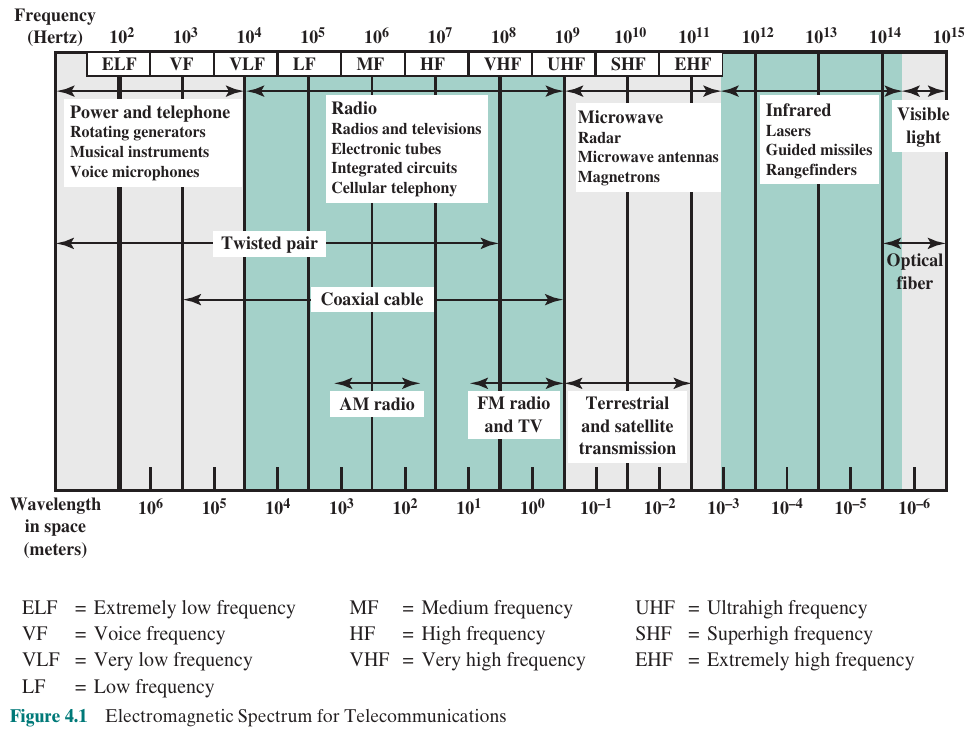
\includegraphics[width=0.9\linewidth]{img/img01}
	\end{center}
\end{frame}

\begin{frame}
	\begin{center}
		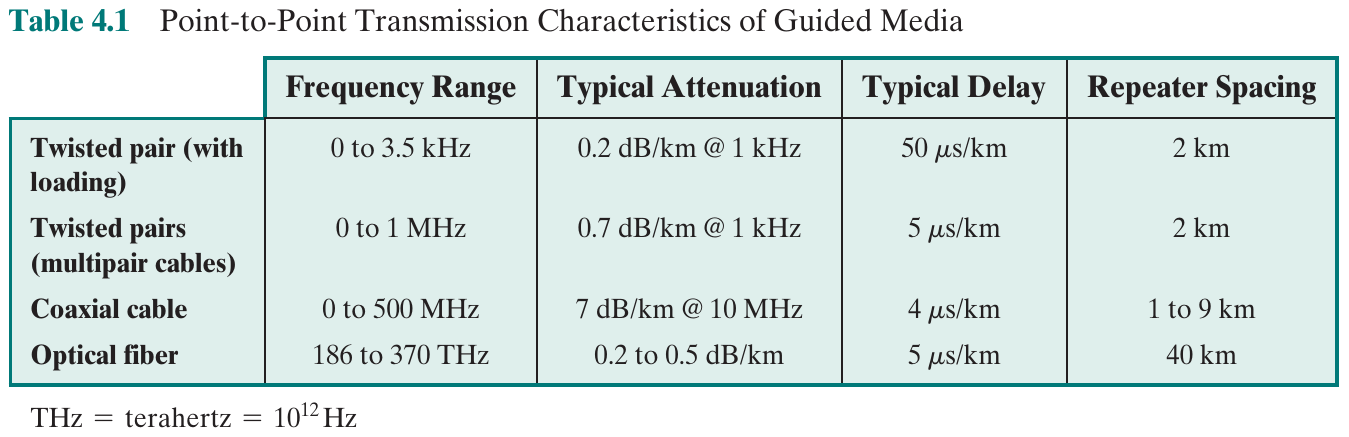
\includegraphics[width=\linewidth]{img/img02}
	\end{center}
\end{frame}

\begin{frame}
	\begin{center}
		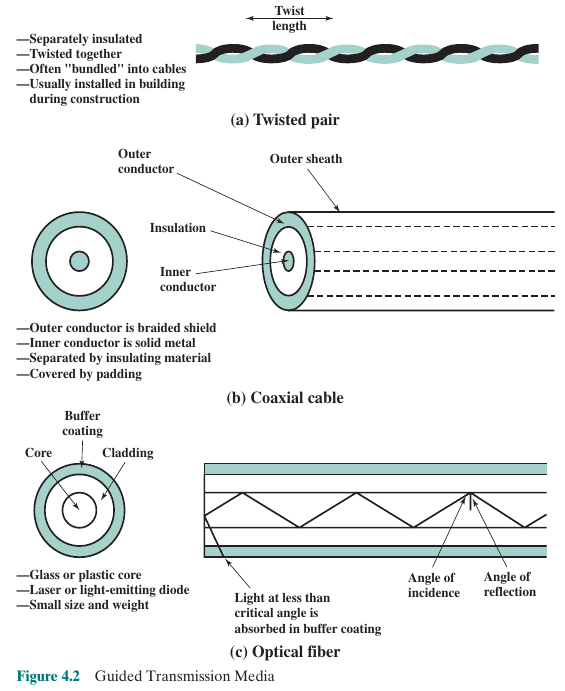
\includegraphics[width=0.5\linewidth]{img/img03a}
	\end{center}
\end{frame}

\begin{frame}
	\frametitle{Twisted Pair}
	\begin{itemize}
		\item Twisted pair is the least expensive and most widely used guided transmission medium
		\begin{center}
			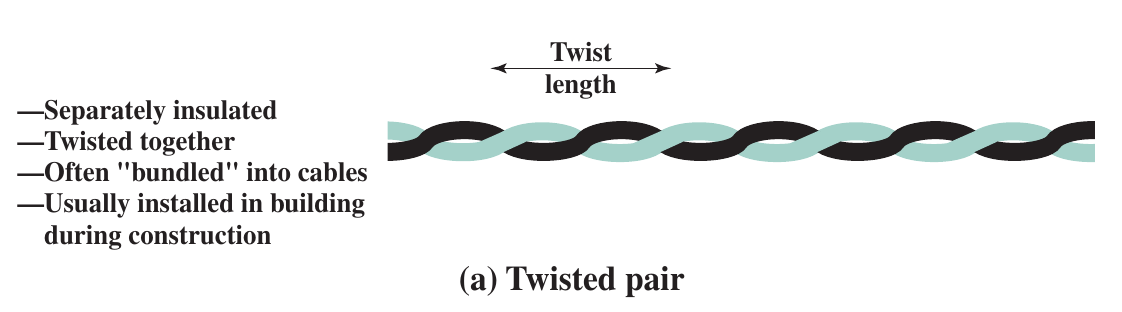
\includegraphics[width=0.8\linewidth]{img/img03}
		\end{center}
		\item Consists of two insulated copper wires arranged in a regular spiral pattern
		\item A wire pair acts as a single communication link
		\item Pairs are bundled together into a cable
		\item Most commonly used in the telephone network and for communications within buildings
	\end{itemize}
\end{frame}

\begin{frame}
	\begin{center}
		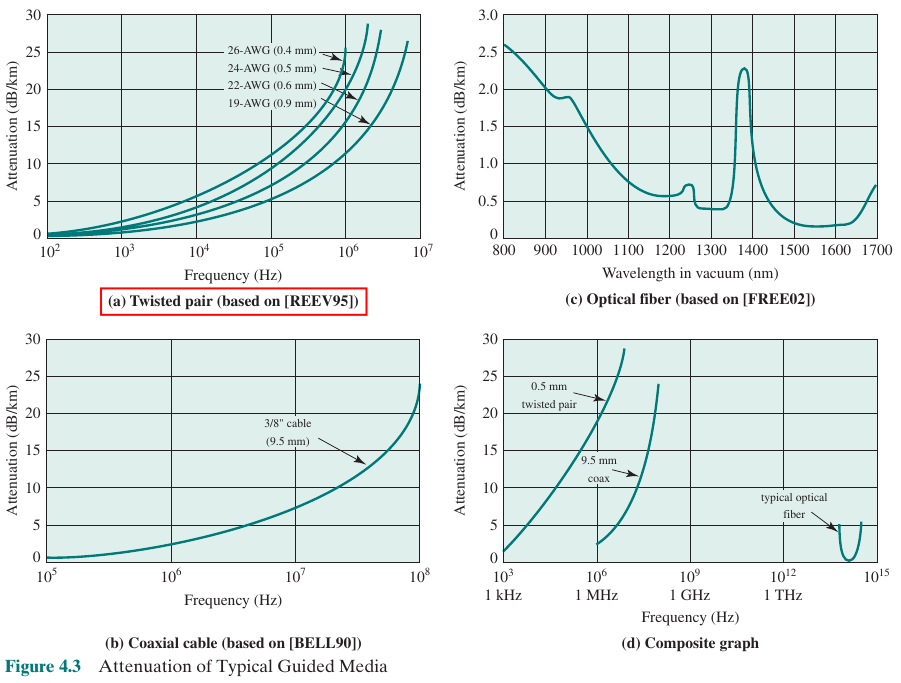
\includegraphics[width=0.8\linewidth]{img/img06}
	\end{center}
\end{frame}

\begin{frame}
	\frametitle{Unshielded and Shielded Twisted Pair}
	\begin{enumerate}
		\item Unshielded Twisted Pair (UTP)
		\begin{itemize}
			\item  Consists of one or more twisted-pair cables, typically enclosed within an overall thermoplastic jacket which provides no electromagnetic shielding
			\item Ordinary telephone wire
			\item Subject to external electromagnetic interference
			\item The tighter the twisting, the higher the supported transmission rate and the greater the cost per meter
		\end{itemize}
		\item Shielded Twisted Pair (STP)
		\begin{itemize}
			\item Has metal braid or sheathing that reduces interference
			\item Provides better performance at higher data rates
			\item More expensive
		\end{itemize}
	\end{enumerate}	
\end{frame}

\begin{frame}
	\begin{center}
		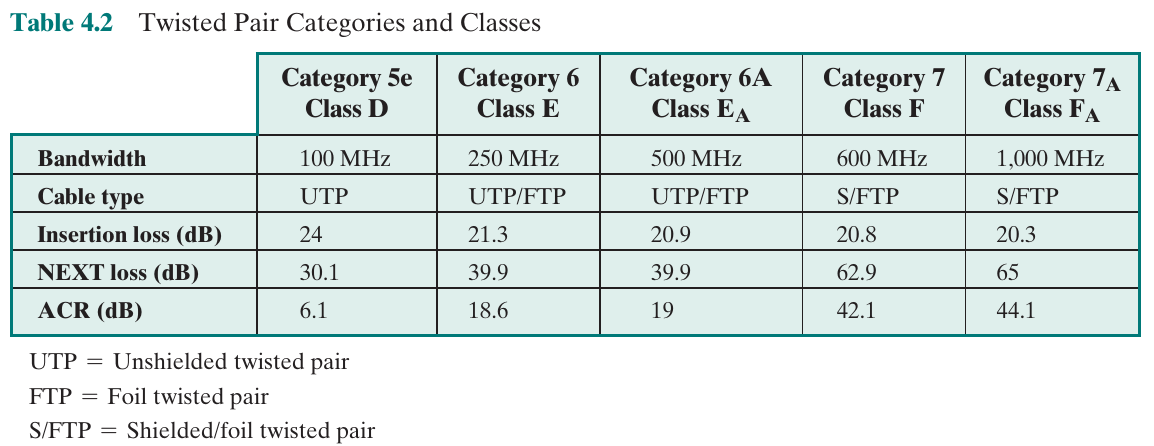
\includegraphics[width=\linewidth]{img/img07}
	\end{center}
\end{frame}

\begin{frame}
	\frametitle{Twisted Pair}
	\begin{center}
		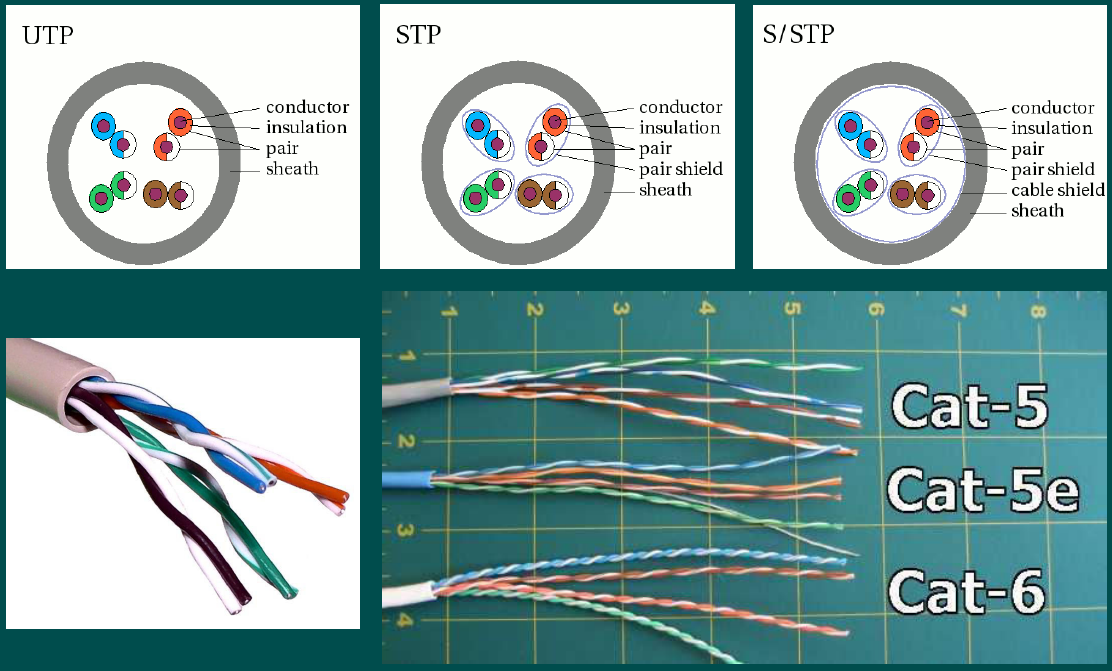
\includegraphics[width=\linewidth]{img/img08}
	\end{center}
\end{frame}

\begin{frame}
	\frametitle{Near-End Crosstalk (NEXT)}
	\begin{itemize}
		\item Coupling of signal from one pair of
		conductors to another
		\begin{itemize}
			\item Conductors may be the metal pins in a connector or wire pairs in a cable
		\end{itemize}
		\item Near end refers to coupling that takes place when the transmit signal entering the link couples back to the receive conductor pair at that same end of the link
		\item Greater NEXT loss magnitudes are associated with less crosstalk noise
	\end{itemize}
\end{frame}

\begin{frame}
	\begin{center}
		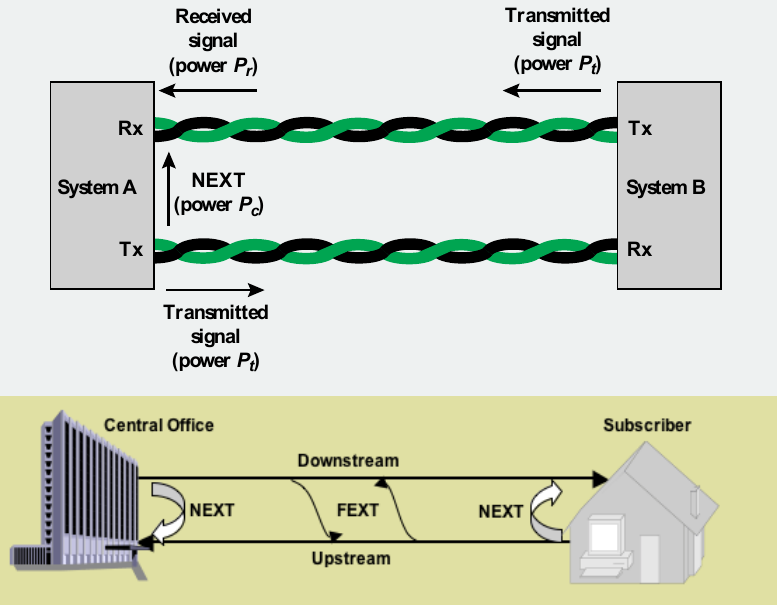
\includegraphics[width=0.8\linewidth]{img/img09}
	\end{center}
\end{frame}

\begin{frame}
	\begin{center}
		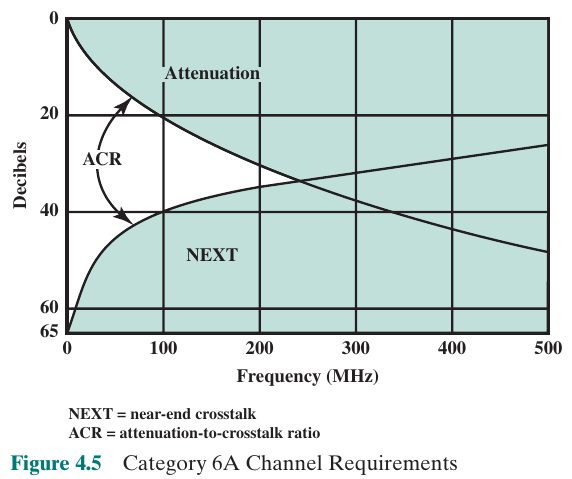
\includegraphics[width=0.7\linewidth]{img/img10}
	\end{center}
\end{frame}

\begin{frame}
	\frametitle{Coaxial Cabel}
	\begin{itemize}
		\item Coaxial cable can be used over longer distances and support more stations on a shared line than twisted pair
		\begin{center}
			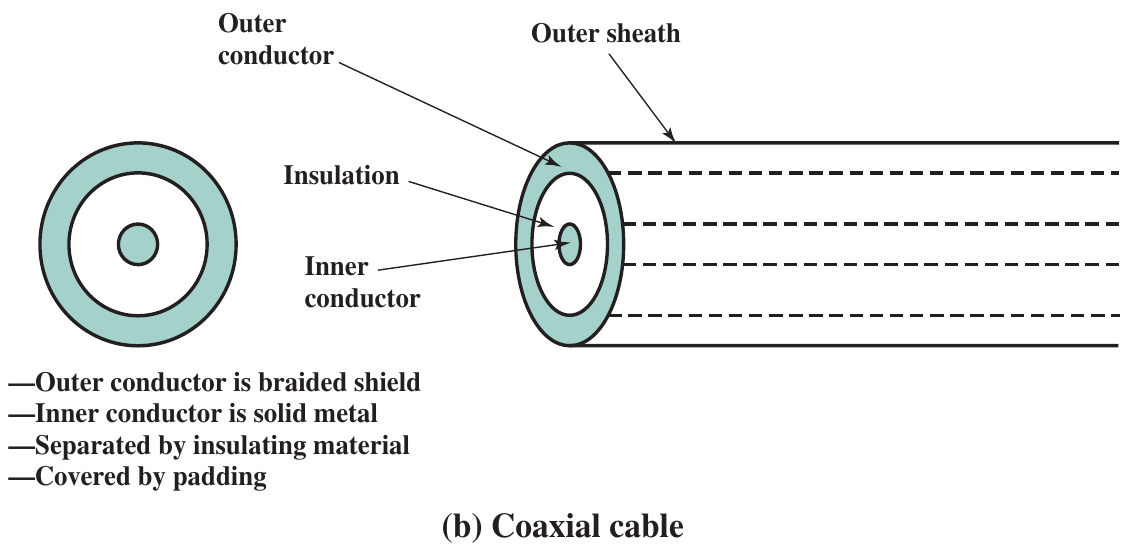
\includegraphics[width=0.5\linewidth]{img/img04}
		\end{center}
		\item Consists of a hollow outer cylindrical conductor that surrounds a single inner wire conductor
		\item Is a versatile transmission medium used in a wide variety of applications
		\item Used for TV distribution, long distance telephone transmission and LANs
	\end{itemize}
\end{frame}

\begin{frame}
	\frametitle{Coaxial Cable - Transmission Characteristics}
	\begin{itemize}
		\item Frequency characteristics superior to twisted pair
		\item Performance limited by attenuation and noise
		\item Analog signals
		\begin{itemize}
			\item  Amplifiers are needed every few kilometers - closer if higher frequency
			\item Usable spectrum extends up to 500MHz
		\end{itemize}
		\item Digital signals
		\begin{itemize}
			\item Repeater every 1 km - closer for higher data rates
		\end{itemize}
	\end{itemize}
	\begin{center}
		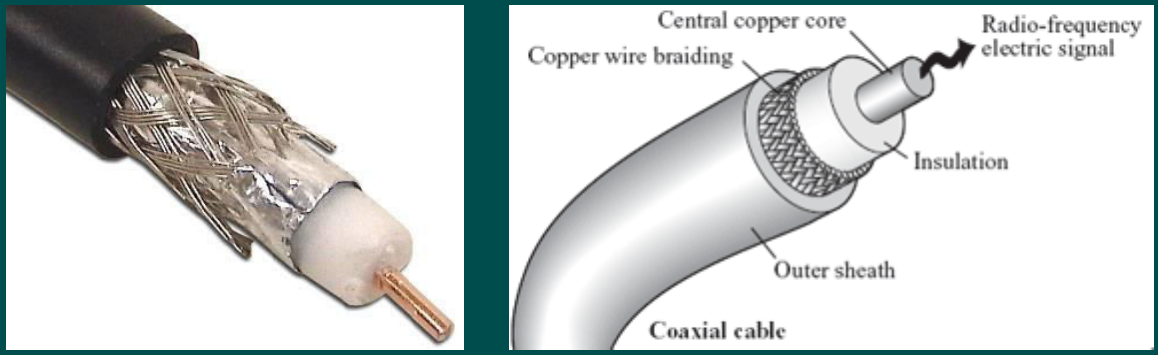
\includegraphics[width=0.7\linewidth]{img/img11}
	\end{center}
\end{frame}

\begin{frame}
	\begin{center}
		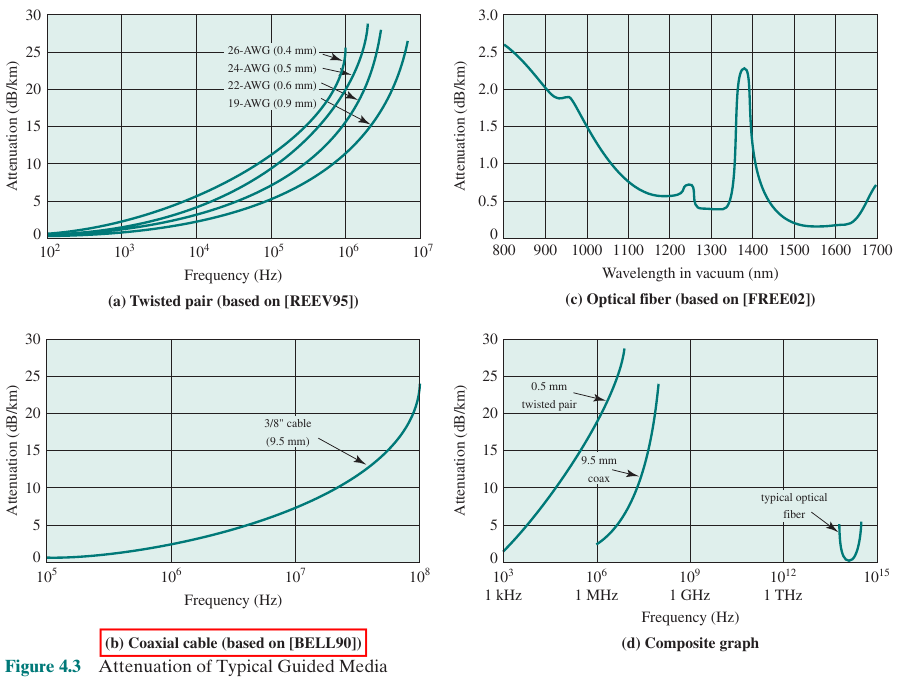
\includegraphics[width=0.8\linewidth]{img/img12}
	\end{center}
\end{frame}

\begin{frame}
	\frametitle{Optical Fiber}
	\begin{itemize}
		\item Optical fiber is a thin flexible medium capable of guiding an optical ray
		\begin{center}
			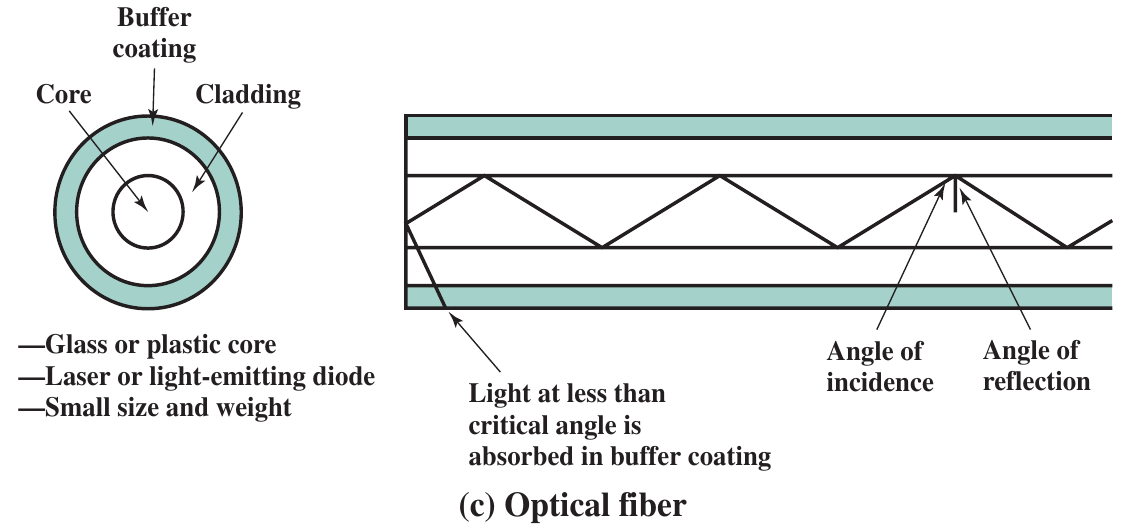
\includegraphics[width=0.5\linewidth]{img/img05}
		\end{center}
		\item Various glasses and plastics can be used to make optical fibers
		\item Has a cylindrical shape with three sections – core, cladding, jacket
		\item Widely used in long distance telecommunications
		\item Performance, price and advantages have made it popular to use
	\end{itemize}
\end{frame}

\begin{frame}{Optical Fiber}
	\begin{center}
		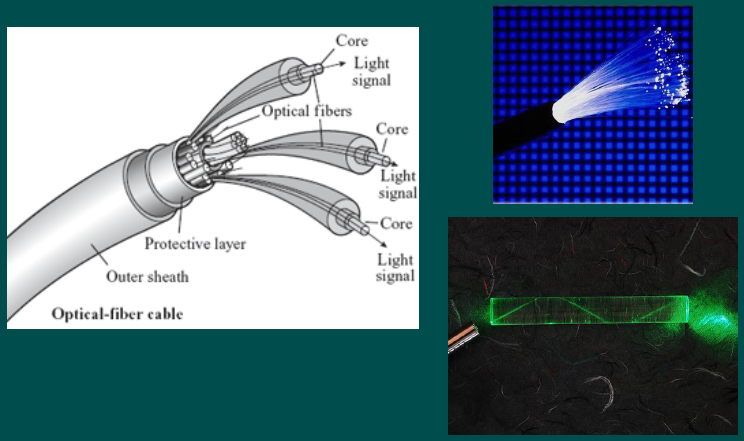
\includegraphics[width=\linewidth]{img/img13}
	\end{center}
\end{frame}

\begin{frame}
	\frametitle{Optical Fiber - Benefits}
	\begin{itemize}
		\item Greater capacity
		\begin{itemize}
			\item Data rates of hundreds of Gbps over tens of kilometers have been demonstrated
		\end{itemize}
		\item Smaller size and lighter weight
		\begin{itemize}
			\item Considerably thinner than coaxial or twisted pair cable
			\item Reduces structural support requirements
		\end{itemize}
		\item Lower attenuation
		\item Electromagnetic isolation
		\begin{itemize}
			\item Not vulnerable to interference, impulse noise, or crosstalk
			\item High degree of security from eavesdropping
		\end{itemize}
		\item Greater repeater spacing
		\begin{itemize}
			\item Lower cost and fewer sources of error
		\end{itemize}
	\end{itemize}
\end{frame}

\begin{frame}
	\frametitle{Categories of Application}
	\begin{itemize}
		\item Five basic categories of application have become important for optical fiber:
		\begin{itemize}
			\item Long-haul trunks
			\item Metropolitan trunks
			\item Rural exchange trunks
			\item Subscriber loops
			\item Local area networks
		\end{itemize}
	\end{itemize}
\end{frame}

\begin{frame}
	\begin{center}
		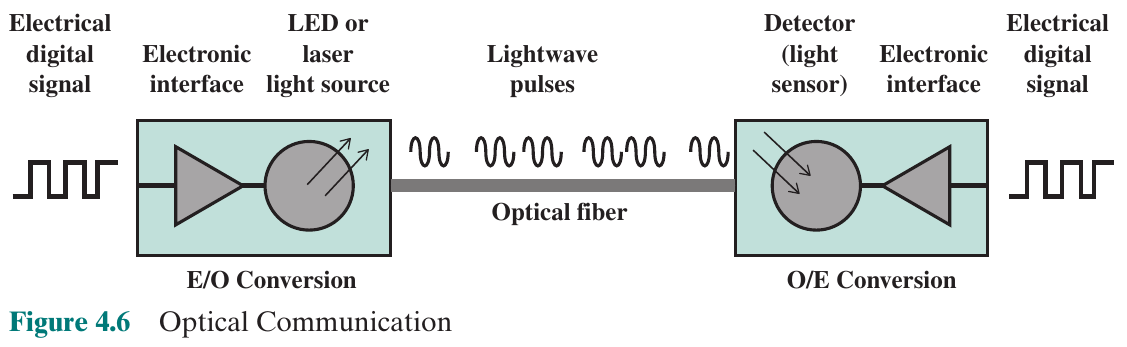
\includegraphics[width=\linewidth]{img/img14}
	\end{center}
\end{frame}

\begin{frame}
	\begin{center}
		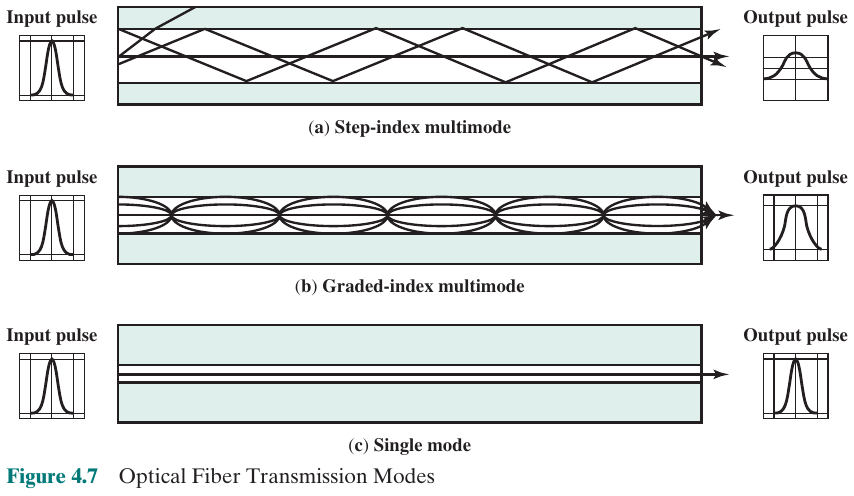
\includegraphics[width=\linewidth]{img/img15}
	\end{center}
\end{frame}

\begin{frame}
	\begin{center}
		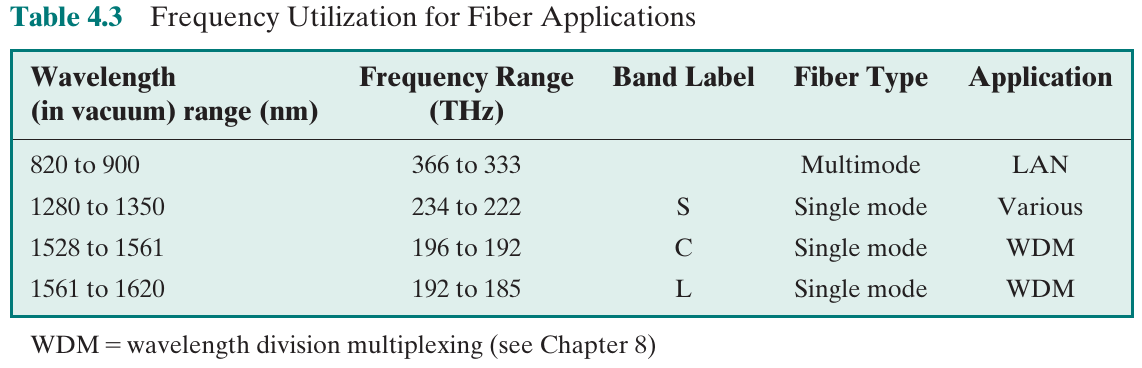
\includegraphics[width=\linewidth]{img/img16}
	\end{center}
\end{frame}

\begin{frame}
	\begin{center}
		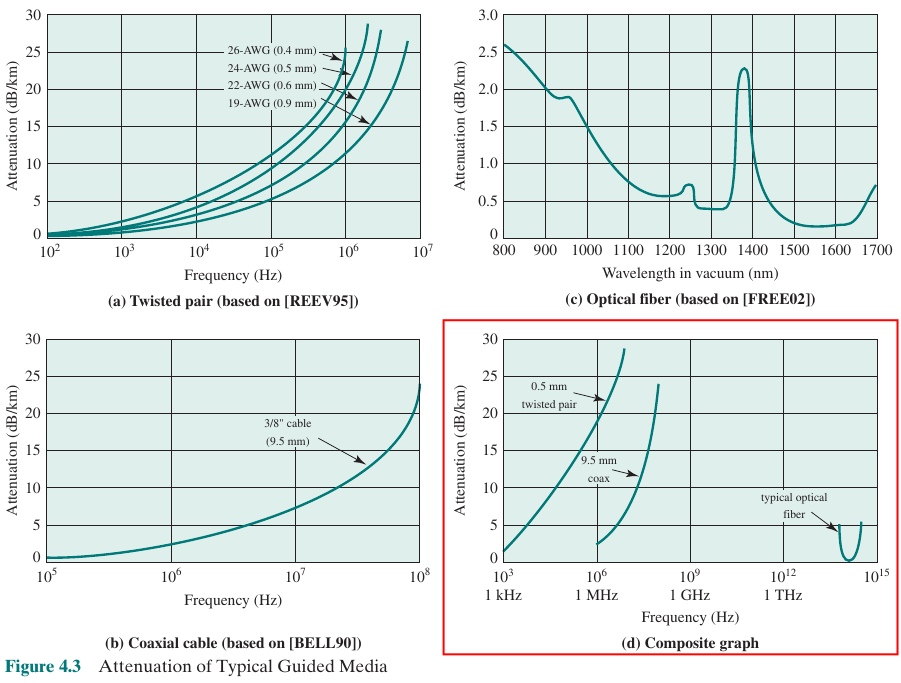
\includegraphics[height=0.9\textheight]{img/img17}
	\end{center}
\end{frame}

\begin{frame}
	\frametitle{Wireless Transmission Frequencies}
	\begin{itemize}
		\item 1GHz to 40GHz
		\begin{itemize}
			\item Referred to as microwave frequencies
			\item Highly directional beams are possible
			\item Suitable for point to point transmissions
			\item Also used for satellite communications
		\end{itemize}
		\item 30 MHz to 1 GHz
		\begin{itemize}
			\item Suitable for omnidirectional applications
			\item Referred to as the radio range
		\end{itemize}
		\item $ 3 \times 10^{11} $ Hz to $ 2 \times 10^{14} $ Hz
		\begin{itemize}
			\item Infrared portion of the spectrum
			\item Useful to local point-to-point and multipoint applications within confined areas
		\end{itemize}
	\end{itemize}
\end{frame}

\begin{frame}
	\frametitle{Antennas}
	\begin{itemize}
		\item Electrical conductor or system of conductors used to radiate or collect electromagnetic energy
		\item Radio frequency electrical energy from the transmitter is converted into electromagnetic energy by the antenna and radiated into the surrounding environment
		\item Reception occurs when the electromagnetic signal intersects the antenna
		\item In two way communication, the same antenna can be used for both transmission and reception
	\end{itemize}
\end{frame}

\begin{frame}
	\frametitle{Radiation Pattern}
	\begin{itemize}
		\item Power radiated in all directions
		\begin{itemize}
			\item Does not perform equally well in all directions
		\end{itemize}
		\item Radiation pattern
		\begin{itemize}
			\item A graphical representation of the radiation properties of an antenna as a function of space coordinates
		\end{itemize}
		\item Isotropic antenna
		\begin{itemize}
			\item A point in space that radiates power in all directions equally
			\item Actual radiation pattern is a sphere with the antenna at the center
		\end{itemize}
	\end{itemize}
\end{frame}

\begin{frame}
	\begin{center}
		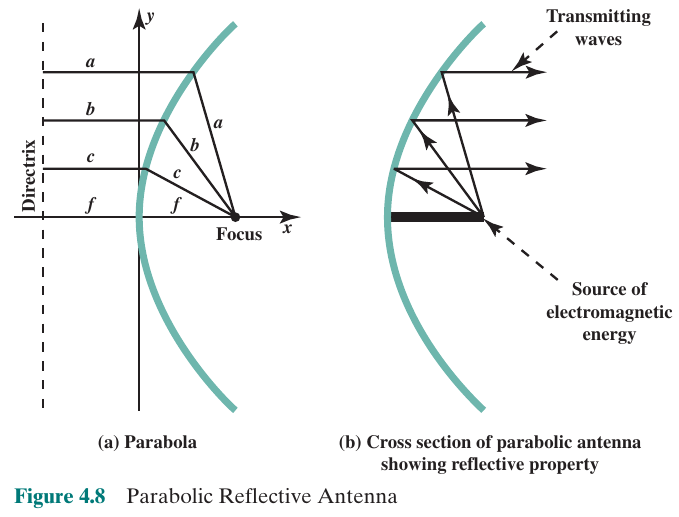
\includegraphics[height=0.9\textheight]{img/img18}
	\end{center}
\end{frame}

\begin{frame}
	\frametitle{Antenna Gain}
	\begin{itemize}
		\item A measure of the directionality of an antenna
		\item Defined as the power output in a particular direction versus that produced by an isotropic antenna
		\item Measured in decibels (dB)
		\item The increased power radiated in a given direction is at the expense of other directions
		\item Effective area of an antenna is related to the physical size of the antenna and to its shape
	\end{itemize}
\end{frame}

\begin{frame}
	\frametitle{Terrestrial Microwave}
	\begin{itemize}
		\item Most common type is the parabolic “dish”
		\item Typical size is about 3 m in diameter
		\item Antenna is fixed rigidly and focuses a narrow beam to achieve line-of-sight transmission to the receiving antenna
		\item Usually located at substantial heights above ground level
		\item A series of microwave relay towers is used to achieve long-distance transmission
	\end{itemize}
\end{frame}

\begin{frame}
	\frametitle{Terrestrial Microwave Applications}
	\begin{itemize}
		\item Used for long haul telecommunications service as an alternative to coaxial cable or optical fiber
		\item Used for both voice and TV transmission
		\item Fewer repeaters but requires line-of-sight transmission
		\item 1 - 40 GHz frequencies, with higher frequencies having higher data rates
		\item Main source of loss is attenuation caused mostly by distance, rainfall and interference
	\end{itemize}
\end{frame}

\begin{frame}
	\begin{center}
		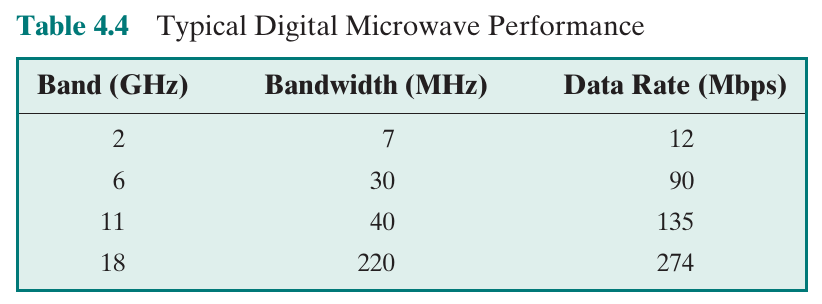
\includegraphics[width=0.9\linewidth]{img/img19}
	\end{center}
\end{frame}

\begin{frame}
	\frametitle{Satellite Microwave}
	\begin{itemize}
		\item A communication satellite is in effect a microwave relay station
		\item Used to link two or more ground stations
		\item Receives transmissions on one frequency band, amplifies or repeats the signal, and transmits it on another frequency
		\begin{itemize}
			\item Frequency bands are called transponder channels
		\end{itemize}
	\end{itemize}
\end{frame}

\begin{frame}
	\begin{center}
		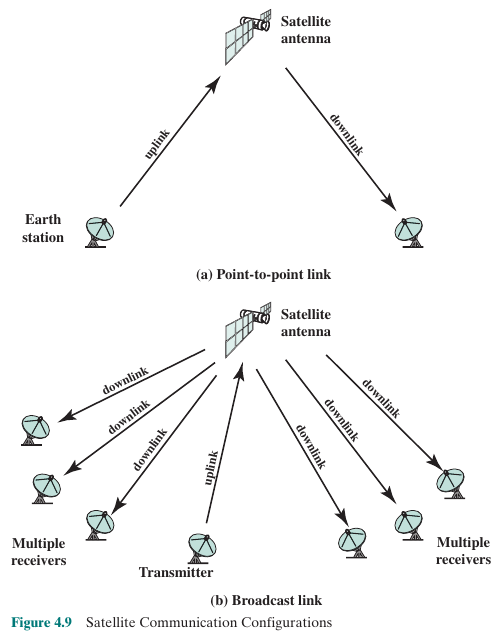
\includegraphics[height=0.9\textheight]{img/img20}
	\end{center}
\end{frame}

\begin{frame}
	\frametitle{Satellite Microwave Applications}
	Most important applications for satellites are:
	\begin{itemize}
		\item Long-distance telephone transmission
		\begin{itemize}
			\item Is the optimum medium for high-usage international trunks
		\end{itemize}
		\item Private business networks
		\begin{itemize}
			\item Satellite providers can divide capacity into channels and lease these channels to individual business users
		\end{itemize}
		\item Television distribution
		\begin{itemize}
			\item Programs are transmitted to the satellite then broadcast down to a number of stations which then distribute the programs to individual viewers
			\item Direct Broadcast Satellite (DBS) transmits video signals directly to the home user
		\end{itemize}
		\item Global positioning
		\begin{itemize}
			\item Navstar Global Positioning System (GPS)
		\end{itemize}
	\end{itemize}
\end{frame}

\begin{frame}
	\begin{center}
		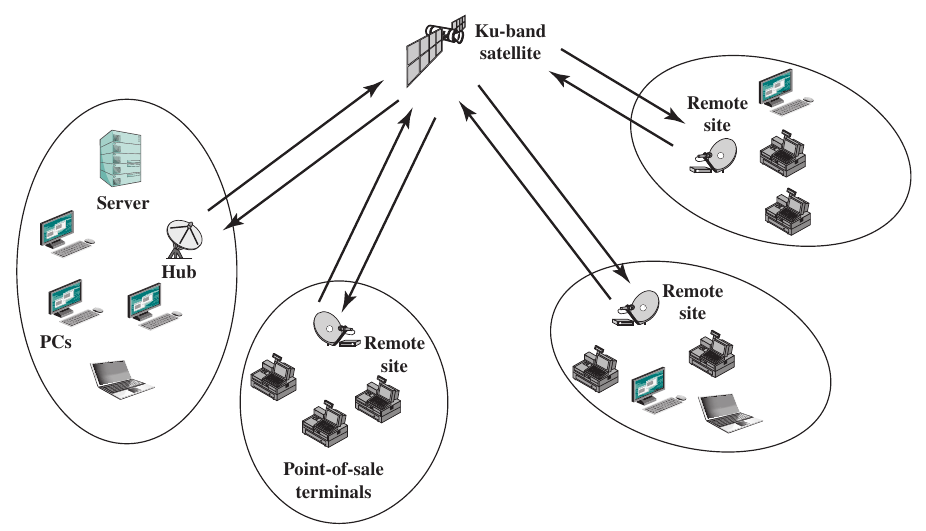
\includegraphics[height=0.8\textheight]{img/img21}
	\end{center}
\end{frame}

\begin{frame}
	\frametitle{Transmission Characteristics}
	\begin{itemize}
		\item The optimum frequency range for satellite transmission is 1 to 10 GHz
		\begin{itemize}
			\item Below 1 GHz there is significant noise from natural sources
			\item Above 10 GHz the signal is severely attenuated by atmospheric absorption and precipitation
		\end{itemize}
		\item Satellites use a frequency bandwidth range of 5.925 to 6.425 GHz from earth to satellite (uplink) and a range of 3.7 to 4.2 GHz from satellite to earth (downlink)
		\begin{itemize}
			\item This is referred to as the 4/6-GHz band
			\item Because of saturation the 12/14-GHz band has been developed
		\end{itemize}
	\end{itemize}
\end{frame}

\begin{frame}
	\frametitle{Broadcast Radio}
	\begin{itemize}
		\item Broadcast radio is omnidirectional and microwave is directional
		\item Radiois the term used to encompass frequencies in the range of 3kHz to 300GHz
		\item Broadcast radio (30MHz - 1GHz) covers:
		\begin{itemize}
			\item FM radio and UHF and VHF television band
			\item Data networking applications
		\end{itemize}
		\item Limited to
		line of sight
		\item Suffers from multipath interference
		\begin{itemize}
			\item Reflections from land, water, man-made objects
		\end{itemize}
	\end{itemize}
\end{frame}

\begin{frame}
	\frametitle{Infrared}
	\begin{itemize}
		\item Achieved using transceivers that modulate noncoherent infrared light
		\item Transceivers must be within line of sight of each other directly or via reflection
		\item Does not penetrate walls
		\item No licensing is required
		\item No frequency allocation issues
	\end{itemize}
\end{frame}

\begin{frame}
	\begin{center}
		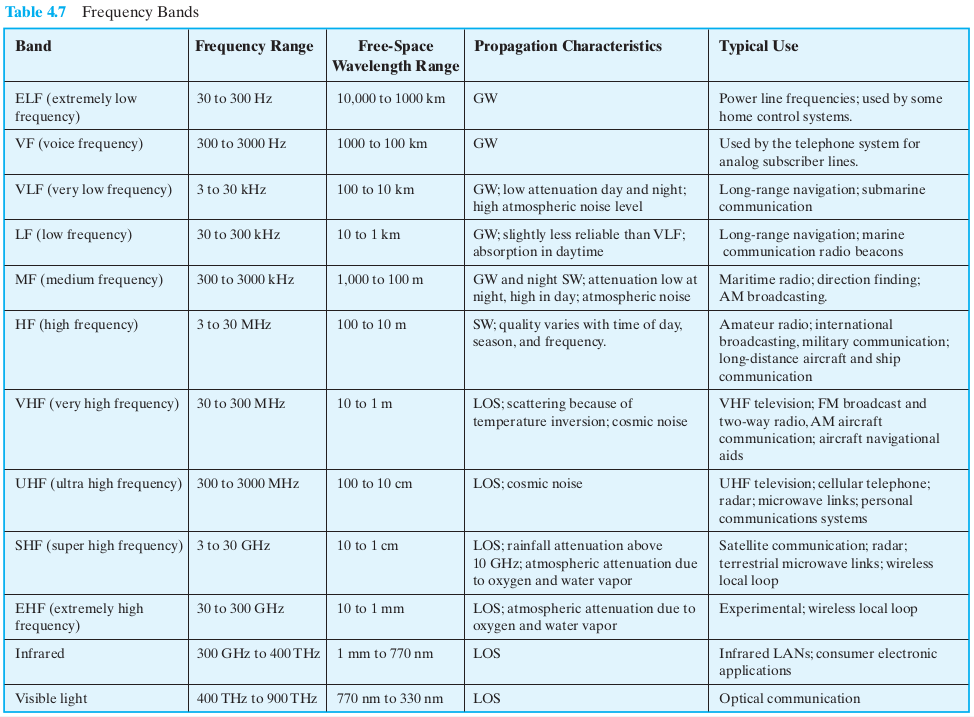
\includegraphics[height=0.8\textheight]{img/img22}
	\end{center}
\end{frame}

\begin{frame}
	\begin{center}
		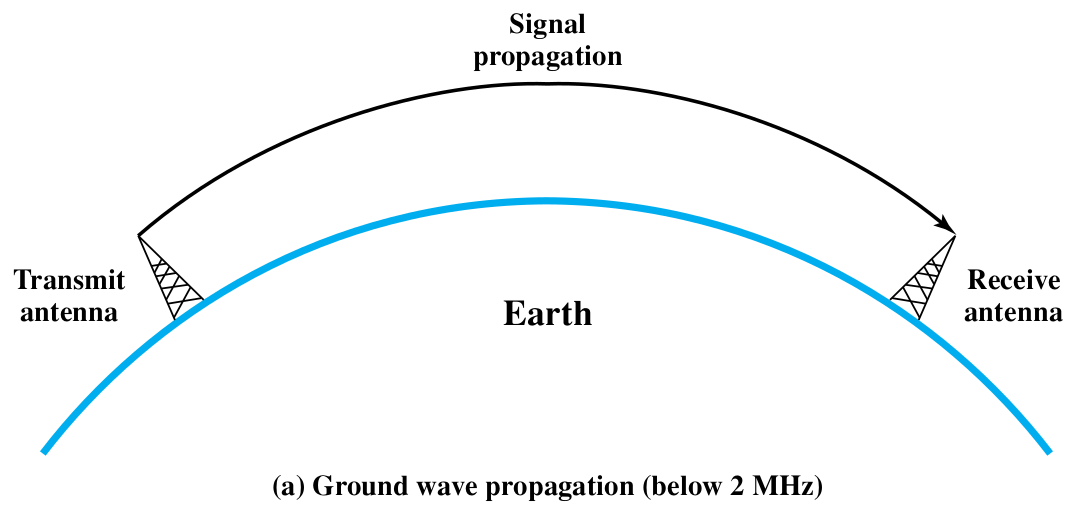
\includegraphics[height=0.4\textheight]{img/img23}
	\end{center}
	\begin{itemize}
		\item Ground wave propagation follows the contour of the earth and can propagate distances well over the visual horizon
		\item This effect is found in frequencies up to about 2 MHz
		\item The best known example of ground wave communication is AM radio
	\end{itemize}
\end{frame}

\begin{frame}
	\begin{center}
		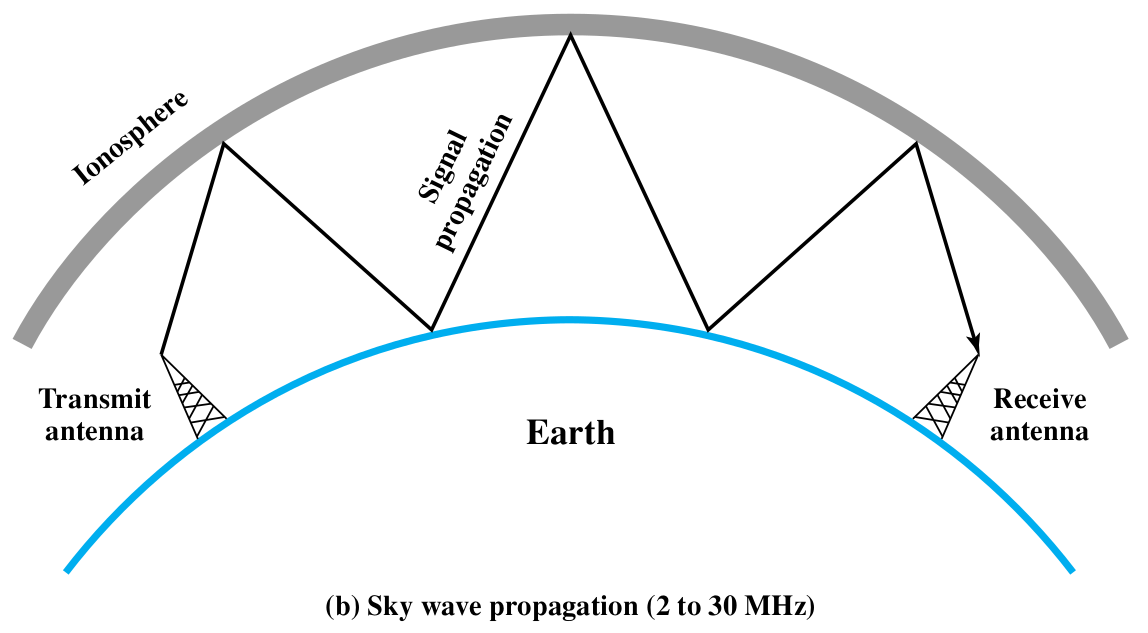
\includegraphics[height=0.4\textheight]{img/img24}
	\end{center}
	\begin{itemize}
		\item Sky wave propagation is used for amateur radio and international broadcasts such as BBC and Voice of America
		\item A signal from an earth based antenna is reflected from the ionized layer of the upper atmosphere back down to earth
		\item Sky wave signals can travel through a number of hops, bouncing back and forth between the ionosphere and the earth's surface
	\end{itemize}
\end{frame}

\begin{frame}
	\begin{center}
		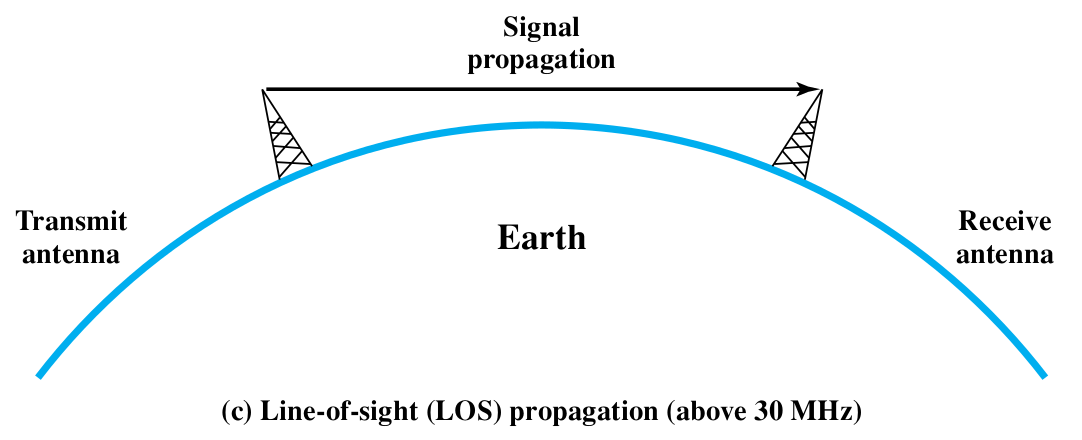
\includegraphics[height=0.4\textheight]{img/img25}
	\end{center}
	\begin{itemize}
		\item Ground and sky wave propagation modes do not operate above 30MHz - - communication must be by line of sight
	\end{itemize}
\end{frame}

\begin{frame}
	\frametitle{Refraction}
	\begin{itemize}
		\item Occurs because the velocity of an electromagnetic wave is a function of the density of the medium through which it travels
		\item $ 3 \times 10^8 $ m/s in a vacuum, less in anything else The speed changes with movement between a medium of one density to a medium of another densit
		\item Index of refraction (refractive index)
		\begin{itemize}
			\item The sine of the angle of incidence divided by the sine of the angle of refraction
			\item Is also equal to the ratio of the respective velocities in the two media
			\item Varies with wavelength
		\end{itemize}
		\item Gradual bending
		\begin{itemize}
			\item Density of atmosphere decreases with height, resulting in bending of radio waves toward the earth
		\end{itemize}
	\end{itemize}
\end{frame}

\begin{frame}
	\begin{center}
		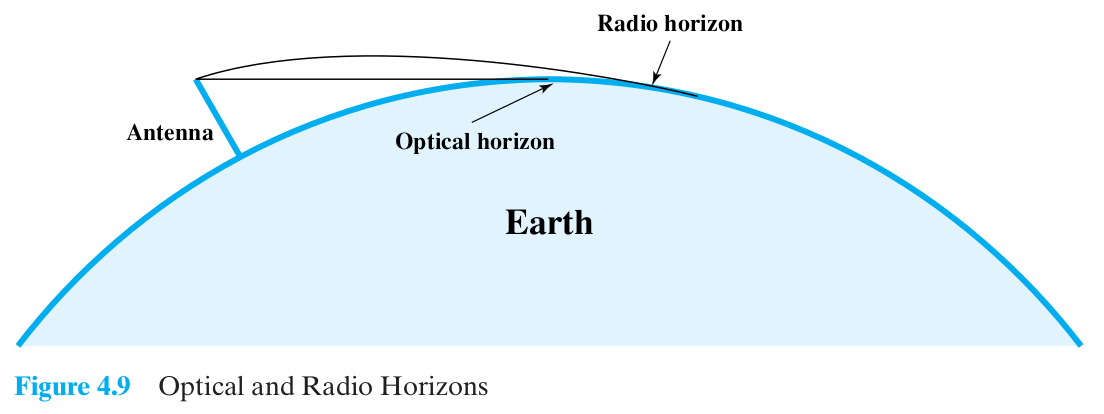
\includegraphics[width=\linewidth]{img/img26}
	\end{center}
\end{frame}

\begin{frame}
	\frametitle{Line-of-Sight Transmission}
	\begin{itemize}
		\item Free space loss
	\end{itemize}
\end{frame}
%-----------------------
%  Tugas
%-----------------------

\begin{frame}
	\frametitle{Tugas Mandiri}
	\begin{itemize}
		\item Stallings, W. (2014). Data and Computer Communications, 10th Edition, New Jersey: Upper Saddle River\\
		\begin{itemize}
			\item Chapter 2 Protocol Architecture, TCP/IP, and Internet-Based Applications
		\end{itemize}
		\item Gupta, P. C. (2006). Data Communications and Computer Networks. New Delhi: Prentice Hall of India\\
		\begin{itemize}
			\item Section 6.8 Layered Architecture of the OSI Reference Model.
			\item Section 6.14.1 TCP/IP
		\end{itemize}
		\item Tanenbaum, A. S. \& Wetherall, D. J. (2013). Computer Networks, Fifth Edition. London: Pearson.\\
		\begin{itemize}
			\item Section 3.1 Protocol Hierarchies
		\end{itemize}
	\end{itemize}
\end{frame}

\begin{frame}
	\frametitle{Tugas Terstruktur}
	\textbf{Tampilkan Tugas 2}
\end{frame}

\end{document}
